% Options for packages loaded elsewhere
\PassOptionsToPackage{unicode}{hyperref}
\PassOptionsToPackage{hyphens}{url}
%

\documentclass[a4paper
]{article}
\usepackage{amsmath,amssymb}
\usepackage{lmodern}
\usepackage{iftex}
\usepackage{geometry}
\ifPDFTeX
  \usepackage[T1]{fontenc}
  \usepackage[utf8]{inputenc}
  \usepackage{textcomp} % provide euro and other symbols
\else % if luatex or xetex
  \usepackage{unicode-math}
  \defaultfontfeatures{Scale=MatchLowercase}
  \defaultfontfeatures[\rmfamily]{Ligatures=TeX,Scale=1}
\fi
% Use upquote if available, for straight quotes in verbatim environments
\IfFileExists{upquote.sty}{\usepackage{upquote}}{}
\IfFileExists{microtype.sty}{% use microtype if available
  \usepackage[]{microtype}
  \UseMicrotypeSet[protrusion]{basicmath} % disable protrusion for tt fonts
}{}
\makeatletter
\@ifundefined{KOMAClassName}{% if non-KOMA class
  \IfFileExists{parskip.sty}{%
    \usepackage{parskip}
  }{% else
    \setlength{\parindent}{0pt}
    \setlength{\parskip}{6pt plus 2pt minus 1pt}}
}{% if KOMA class
  \KOMAoptions{parskip=half}}
\makeatother
\usepackage{xcolor}
\IfFileExists{xurl.sty}{\usepackage{xurl}}{} % add URL line breaks if available
\IfFileExists{bookmark.sty}{\usepackage{bookmark}}{\usepackage{hyperref}}
\hypersetup{
  pdftitle={ADA lecture notes},
  hidelinks,
  pdfcreator={LaTeX via pandoc}}
\urlstyle{same} % disable monospaced font for URLs
\usepackage{color}
\usepackage{fancyvrb}
\newcommand{\VerbBar}{|}
\newcommand{\VERB}{\Verb[commandchars=\\\{\}]}
\DefineVerbatimEnvironment{Highlighting}{Verbatim}{commandchars=\\\{\}}
% Add ',fontsize=\small' for more characters per line
\newenvironment{Shaded}{}{}
\newcommand{\AlertTok}[1]{\textcolor[rgb]{1.00,0.00,0.00}{\textbf{#1}}}
\newcommand{\AnnotationTok}[1]{\textcolor[rgb]{0.38,0.63,0.69}{\textbf{\textit{#1}}}}
\newcommand{\AttributeTok}[1]{\textcolor[rgb]{0.49,0.56,0.16}{#1}}
\newcommand{\BaseNTok}[1]{\textcolor[rgb]{0.25,0.63,0.44}{#1}}
\newcommand{\BuiltInTok}[1]{#1}
\newcommand{\CharTok}[1]{\textcolor[rgb]{0.25,0.44,0.63}{#1}}
\newcommand{\CommentTok}[1]{\textcolor[rgb]{0.38,0.63,0.69}{\textit{#1}}}
\newcommand{\CommentVarTok}[1]{\textcolor[rgb]{0.38,0.63,0.69}{\textbf{\textit{#1}}}}
\newcommand{\ConstantTok}[1]{\textcolor[rgb]{0.53,0.00,0.00}{#1}}
\newcommand{\ControlFlowTok}[1]{\textcolor[rgb]{0.00,0.44,0.13}{\textbf{#1}}}
\newcommand{\DataTypeTok}[1]{\textcolor[rgb]{0.56,0.13,0.00}{#1}}
\newcommand{\DecValTok}[1]{\textcolor[rgb]{0.25,0.63,0.44}{#1}}
\newcommand{\DocumentationTok}[1]{\textcolor[rgb]{0.73,0.13,0.13}{\textit{#1}}}
\newcommand{\ErrorTok}[1]{\textcolor[rgb]{1.00,0.00,0.00}{\textbf{#1}}}
\newcommand{\ExtensionTok}[1]{#1}
\newcommand{\FloatTok}[1]{\textcolor[rgb]{0.25,0.63,0.44}{#1}}
\newcommand{\FunctionTok}[1]{\textcolor[rgb]{0.02,0.16,0.49}{#1}}
\newcommand{\ImportTok}[1]{#1}
\newcommand{\InformationTok}[1]{\textcolor[rgb]{0.38,0.63,0.69}{\textbf{\textit{#1}}}}
\newcommand{\KeywordTok}[1]{\textcolor[rgb]{0.00,0.44,0.13}{\textbf{#1}}}
\newcommand{\NormalTok}[1]{#1}
\newcommand{\OperatorTok}[1]{\textcolor[rgb]{0.40,0.40,0.40}{#1}}
\newcommand{\OtherTok}[1]{\textcolor[rgb]{0.00,0.44,0.13}{#1}}
\newcommand{\PreprocessorTok}[1]{\textcolor[rgb]{0.74,0.48,0.00}{#1}}
\newcommand{\RegionMarkerTok}[1]{#1}
\newcommand{\SpecialCharTok}[1]{\textcolor[rgb]{0.25,0.44,0.63}{#1}}
\newcommand{\SpecialStringTok}[1]{\textcolor[rgb]{0.73,0.40,0.53}{#1}}
\newcommand{\StringTok}[1]{\textcolor[rgb]{0.25,0.44,0.63}{#1}}
\newcommand{\VariableTok}[1]{\textcolor[rgb]{0.10,0.09,0.49}{#1}}
\newcommand{\VerbatimStringTok}[1]{\textcolor[rgb]{0.25,0.44,0.63}{#1}}
\newcommand{\WarningTok}[1]{\textcolor[rgb]{0.38,0.63,0.69}{\textbf{\textit{#1}}}}
\usepackage{graphicx}
\makeatletter
\def\maxwidth{\ifdim\Gin@nat@width>\linewidth\linewidth\else\Gin@nat@width\fi}
\def\maxheight{\ifdim\Gin@nat@height>\textheight\textheight\else\Gin@nat@height\fi}
\makeatother
% Scale images if necessary, so that they will not overflow the page
% margins by default, and it is still possible to overwrite the defaults
% using explicit options in \includegraphics[width, height, ...]{}
\setkeys{Gin}{width=\maxwidth,height=\maxheight,keepaspectratio}
% Set default figure placement to htbp
\makeatletter
\def\fps@figure{htbp}
\makeatother
\setlength{\emergencystretch}{3em} % prevent overfull lines
\providecommand{\tightlist}{%
  \setlength{\itemsep}{0pt}\setlength{\parskip}{0pt}}
\setcounter{secnumdepth}{-\maxdimen} % remove section numbering
\ifLuaTeX
  \usepackage{selnolig}  % disable illegal ligatures
\fi

\title{ADA lecture notes}
\author{}
\date{}

\begin{document}
\maketitle

\hypertarget{analysis-and-design-of-algorithms}{%
\section{Analysis and design of
algorithms}\label{analysis-and-design-of-algorithms}}

These are the notes for analysis and design of algorithms course. The
professor says it'll be an interesting course, let's see about that. I
am using Obsidian and this is an amazing markdown editor! It has a lot
of community plugins. Anyways, study now... xD

\hypertarget{here-is-a-somewhat-detailed-overview.}{%
\subsection{Here is a somewhat detailed
overview.}\label{here-is-a-somewhat-detailed-overview.}}

\begin{enumerate}
\tightlist
\item
  ADA/Lecture 1 : Introduction to the course and grading.
\item
  ADA/Lecture 2 : Mastering Master Theorem
\item
  ADA/Lecture 3 : DAC
\item
  ADA/Lecture 4 : DAC continued
\item
  ADA/Lecture 5 : Last DAC
\end{enumerate}

\hfill\break

\hypertarget{lecture-1}{%
\section{Lecture\textrightarrow1}\label{lecture-1}}

It's like DSA version 2 (in terms of management). Here's the link for
previous year:
\href{https://sites.google.com/iiitd.ac.in/ada2020/lectures}{ADA2020},
\href{https://sites.google.com/iiitd.ac.in/ada22}{ADA2022}. Solutions
and questions in this course are made by the instructor and hence making
it public is not a good idea. So, these notes with stick around the
lectures and maybe sometimes touching things but WILL NOT quote.

\hypertarget{evaluation}{%
\subsection{Evaluation}\label{evaluation}}

\begin{itemize}
\tightlist
\item
  Quizzes : 15\% (n-1)
\item
  Homework Assignments (Theory) : 15\% (group of two)
\item
  Programming Assignments : 10\% (Foobar, No lab hours, Individual)
\item
  Midsem : 30\%
\item
  Endsem : 30\% Both theory
\end{itemize}

\hypertarget{multiplying-large-integers}{%
\subsection{Multiplying large
integers}\label{multiplying-large-integers}}

Input : Two {\(n\)}-digit numbers {\(A\)} and {\(B\)} Output: Product
{\(A \times B\)} Primitive Ops: Add/Multiply two single digit integers
(recall digital circuits adder)

\begin{itemize}
\item
  Classical pen-paper approach:

  \begin{itemize}
  \tightlist
  \item
    At max {\(2n\)} operations per partial product, since {\(n\)}, we
    have {\(2n^{2}\)}
  \item
    Summation of them, {\(2n^{2}\)}
  \item
    Net {\(4n^{2}\)}
  \end{itemize}
\item
  Doing it differently: (Main idea: {\(\frac{n}{2}\)} digits for each
  {\(a,b,c,d\)})

  \begin{itemize}
  \tightlist
  \item
    {\(\overset{a}{\overbrace{56}}\overset{b}{\overbrace{78}} \times \overset{c}{\overbrace{12}}\overset{d}{\overbrace{34}}\)}

    \begin{enumerate}
    \tightlist
    \item
      Compute {\(a.c = 672\)}
    \item
      Compute {\(b.d = 2652\)}
    \item
      Compute {\((a + b)(c + d) = 6164\)}
    \item
      Compute {\(\boxed{3. - 2. - 1.} = 2840\)}
    \item
      Put it all together {\(6720000 + 2652 + 284000\)} (Notice the
      padding)
    \item
      Do it all recursively
    \end{enumerate}
  \item
    Here's the recursive implementation, where
    {\(A = 10^{\frac{n}{2}} \cdot a + b,B = 10^{\frac{n}{2}} \cdot c + d\)}
    and {\(A \times B = 10^{n}ac + 10^{\frac{n}{2}}(ad + bc) + bd\)}

    \begin{enumerate}
    \tightlist
    \item
      Recursively compute {\(a.c\)}
    \item
      Recursively compute {\(b.d\)}
    \item
      Recursively compute {\((a + b) \cdot (c + d)\)} (Karatsuba method,
      otherwise 4 recursive calls)
    \item
      Compute {\(\boxed{3. - 2. - 1.}\)} for each call
    \item
      Pad and add!
    \end{enumerate}
  \end{itemize}
\end{itemize}

\hypertarget{lecture-2}{%
\section{Lecture\textrightarrow2}\label{lecture-2}}

\hypertarget{analysis-the-recurrence-method}{%
\subsection{Analysis: The recurrence
method}\label{analysis-the-recurrence-method}}

{\(T(n) =\)} Runtime of Algorithm {\(1\)} for multiplying two
{\(n\)}-digit numbers\\
Base Case : {\(n = 1,T(n) = c\)} : Multiplying two single digit
numbers\\
Recurrence (for {\(n > 1\)}) : Express {\(T(n)\)} as the runtime of
recursive calls + additional work which maybe done in that call.

Recursively compute each {\(ac,bd,bc,ad\)}, work in this step
{\[\begin{matrix}
{T(n)} & {= \overset{\text{computing\ ac,bd,bc,bd}}{\overbrace{4T\left( \frac{n}{2} \right)}} + \overset{\text{Adding\ 4\ n/2\ (+padded)\ digit\ no.s}}{\overbrace{c_{1} \cdot n}}} \\
{T(1)} & {= \underset{\text{Base\ case}}{\underbrace{c}}} \\
\end{matrix}\]}

Karatsuba's Algorithm (more like optimization) ({\(a + b\)} may have
{\(\frac{n}{2} + 1\)} digits)

\[\begin{matrix}
{T(n)} & {= \overset{\text{n/2+1\ but\ ignore}}{\overbrace{3T\left( \frac{n}{2} \right)}} + \overset{\text{Adding\ a+b,\ multiplying\ each\ other}}{\overbrace{(c_{2} + c_{3}) \cdot n}}} \\
{T(1)} & {= \underset{\text{Base\ case}}{\underbrace{c}}} \\
\end{matrix}\]

\hypertarget{master-method-master-theorem}{%
\subsubsection{Master Method / Master
Theorem}\label{master-method-master-theorem}}

A 'Black-box' method to solve many common recurrences in Algorithm
design (especially DAC)

\textbf{Assumption}: All the recursive calls are made on subproblems of
equal size. (If not, use the proof we will do now)

\textbf{Assumption (for proof)}: Both constants {\(c\)} are equal.

\[\begin{matrix}
{T(n)} & {= {aT\left( \frac{n}{b} \right)} + {c \cdot n^{d}}} \\
{T(1)} & {\leq c} \\
\end{matrix}\]

{\[a \geq 1,b \geq 1,c,d \geq 0\]}{\(a\)} = Number of recursive calls\\
{\(b\)} = Shrinkage factor of subproblem size\\
{\(d\)} = Affects the runtime of the additional work (outside recursion)

Master Theorem (Simpler Version): Prof. says no need to \emph{remember}

\[T(n) = \left\{ \begin{matrix}
{\mathcal{O}(n^{d}\log n),} & {\text{if~}a = b^{d}} \\
{\mathcal{O}(n^{d}),} & {\text{if~}a < b^{d}} \\
{\mathcal{O}(n^{\log_{b}a}),} & {\text{if~}a > b^{d}} \\
\end{matrix} \right.\]

Example: Mergesort, {\(T(n) = 2T(n/2) + c \cdot n\)} so
{\(a = 2,b = 2,d = 1\)}, so case 1. {\(T(n) = \mathcal{O}(n\log n)\)}

Example: Binary search, {\(T(n) = T(n/2) + c \cdot n^{0}\)}, so
{\(a = 1,b = 2,d = 0\)}, so case 1. {\(T(n) = \mathcal{O}(\log n)\)}

Example: Multiplication algorithm1, {\(T(n) = 4T(n/2) + c_{1}n\)}, so
{\(a = 4,b = 2,d = 1\)}, so case 3. {\(\mathcal{O}(n^{\log_{4}2})\)}

Example: Multiplication algorithm (Karatsuba),
{\(T(n) = 3T(n/2) + c_{1}n\)}, so {\(a = 3,b = 2,d = 1\)}, so case 3.
{\(\mathcal{O}(n^{\log_{3}2})\)}

\begin{itemize}
\tightlist
\item
  The calculator uses Strassen Schonenhage:
  {\(\mathcal{O}(n\log n\log\log n)\)}
\item
  New proposed solution: {\(\mathcal{O}(n\log n)\)}
\end{itemize}

\hypertarget{proof-of-master-theorem-simpler-version}{%
\subsection{Proof of master theorem (Simpler
version)}\label{proof-of-master-theorem-simpler-version}}

\textbf{Assumtions}:\\
1. {\(n\)} is a power of {\(b\)} (the shrinkage factor)\\
2. Base case: {\(T(1) = c\)} (same as {\(n^{d}\)})

\textbf{Main technique}:

\begin{itemize}
\tightlist
\item
  Recursion Trees (eww)

  \begin{itemize}
  \tightlist
  \item
    Levels: {\(\boxed{\log_{b}n + 1}\)}
  \item
    Subproblems at level {\(j\)}: {\(\boxed{a^{j}}\)}
  \item
    Subproblem size at level {\(j\)}: {\(\boxed{\frac{n}{b^{j}}}\)}
  \item
    \emph{Total} work done outside recursive calls at level {\(j\)}:
    {\(\boxed{a^{j} \cdot \left( \frac{n}{b^{j}} \right)^{d} \cdot c} = n^{d}\left( \frac{a}{b^{d}} \right)^{j} \cdot c\)}\\
    Should be intuitive from the above equation, Good = {\(a\)}, bad =
    {\(b^{d}\)}, in the end we just sum it all.
  \item
    So, work is sum of total work across all
    levels{\[\sum\limits_{j = 0}^{\log_{b}n + 1}n^{d}\left( \frac{a}{b^{d}} \right)^{j} \cdot c\]}
  \end{itemize}
\end{itemize}

\hypertarget{lecture-3}{%
\section{Lecture\textrightarrow3}\label{lecture-3}}


\includegraphics[width=4.16667in,height=\textheight]{D:/IIITD/Semester4/ADA/Pasted image 20220128134320.png}

\hypertarget{divide-and-conquer-algorithms}{%
\subsection{Divide and Conquer
Algorithms}\label{divide-and-conquer-algorithms}}

\begin{enumerate}
\tightlist
\item
  Divide (break into several parts)
\item
  Conquer (Solve the smallest solvable)
\item
  Combine (subproblems)
\end{enumerate}

\hypertarget{counting-inversions-in-an-array}{%
\subsubsection{Counting Inversions in an
Array}\label{counting-inversions-in-an-array}}

Input: {\(1,3,5,2,4,6\)}\\
Output: {\(3\)}\\
Inversion pairs: {\((3,2),(5,2),(5,4)\)} \{kind of like bubble sort\}\\
Golden Benchmark to get inversions: Sorted array (ascending)\\
Trivial algorithm = {\(\mathcal{O}(n^{2})\)}\\
Today: {\(\mathcal{O}(n\log n)\)}\\
Q. Can we output all inversions in same time above? No, total
{\(O(n^{2})\)} possible invs.

\begin{itemize}
\item
  Key Ideas

  \begin{itemize}
  \tightlist
  \item
    Suppose {\(A\)} is divided in to {\(X\)} and {\(Y\)} (possibly in
    the middle)
  \item
    An inversion pair {\((i,j)\)} is :

    \begin{enumerate}
    \tightlist
    \item
      Left inversion : Both {\((i,j)\)} in {\(X\)}
    \item
      Right inversion : Both {\((i,j)\)} in {\(Y\)}
    \item
      Split inversion : {\(i\)} in {\(X\)} and {\(j\)} in {\(Y\)}
    \end{enumerate}
  \item
    Using recursion get {\((1),(2)\)} and after you get the results,
    count split inversions.
  \item
    Here's the pseudo code
  \end{itemize}

\begin{Shaded}
\begin{Highlighting}[]
\NormalTok{CountInv(array\& A, length n):}
\NormalTok{    if n==1 return 0}
\NormalTok{    X = A[1,2,...n/2], Y=A[n/2+1,...,n]}
\NormalTok{    x = CountInv(X,n/2)}
\NormalTok{    y = CountInv(Y,n/2)}
\NormalTok{    x = CountSplitInv(X,n/2)}
\NormalTok{    return x+y+x}
\NormalTok{Copy}
\end{Highlighting}
\end{Shaded}

  \begin{itemize}
  \tightlist
  \item
    Now, since split inversions wont be affected if we sort each X and Y
    (along the recursive calls) it'll get easier to count inversions. We
    will use this to count split inversions while merging.
    \texttt{count\ +=\ (n/2\ -\ i\ +\ 1)} where {\(i\)} is the iterator
    of {\(X\)} and we are using the combine/merge function. This takes
    advantage of sorting.
  \end{itemize}
\end{itemize}

\hypertarget{lecture-4}{%
\section{Lecture\textrightarrow4}\label{lecture-4}}

\hypertarget{closest-pair-of-points-in-2d}{%
\subsection{Closest pair of points in
2D}\label{closest-pair-of-points-in-2d}}

Input: A set of points with {\(2\)} coordinates\\
Distance {\((d)\)} between two points is \emph{Euclidean distance} in
{\(2D\)}\\
Output: {\((a,b):d(a,b)\)} is minimum\\
Assumption: All points have {\(x\)} and {\(y\)} coordinates (Non
distinct left as exercise)

\textbf{The 1-D case:}\\
Sort the given points, and linearly traverse. So complexity
{\(\mathcal{O}(n\log n)\)}

\textbf{Back to 2D:}\\
{\(P_{x}\)} be the set sorted by x-coordinate\\
{\(P_{y}\)} be the set sorted by y-coordinate (independent of other
coordinate)\\
Now we choose the median using P\_x. Then we have two sets, Q,R on left
and right of the median (assume median on Q).

Recursion:

\begin{enumerate}
\tightlist
\item
  Compute {\(Q_{x},Q_{y},R_{x},R_{y}\)}
\item
  {\((p_{1},q_{1}) = {ClosestPair}(Q_{x},Q_{y})\)}
\item
  {\((p_{2},q_{2}) = {ClosestPair}(R_{x},R_{y})\)}
\item
  Generate the sets {\(Q_{x},Q_{y},R_{x},R_{y}\)} in
  {\(\mathcal{O}(n)\)} time {[}Exercise{]}
\item
  {\((p_{3},q_{3}) = {ClosestSplitPair}(Q,R)\)}
\item
  get minimum of all {\(3\)}
\end{enumerate}

ClosestSplitPair:

\begin{enumerate}
\tightlist
\item
  Our search space will be restricted to {\(\pm \delta\)} where\\
  {\(\delta = \min({ClosestPair}(Q),{ClosestPair}(R))\)}
\item
  Note that this may not return a correct answer if the closest split
  pair does not lie in our restricted search space.
\item
  Calculations, we'll make it {\(\mathcal{O}(n)\)}; now assume the set
  {\(S\)} is the set of points contained in the predefined region.
\item
  Compute {\(S_{y}\)} (sorted by {\(y\)} coordinate) in linear time.
\item
  Traverse the list and apply the 1D algorithm but lookahead
  \textbf{seven} points instead of \textbf{one}. So complexity
  {\(\mathcal{O}(7n) \subseteq \mathcal{O}(n)\)}.

  \begin{itemize}
  \tightlist
  \item
    Proof of correctness of \textbf{seven}
  \item
    We use the fact that our search space is restricted by
    {\(\pm \delta\)} and what is {\(\delta\)}
  \item
    Therefore each box below will have at most one point\\
    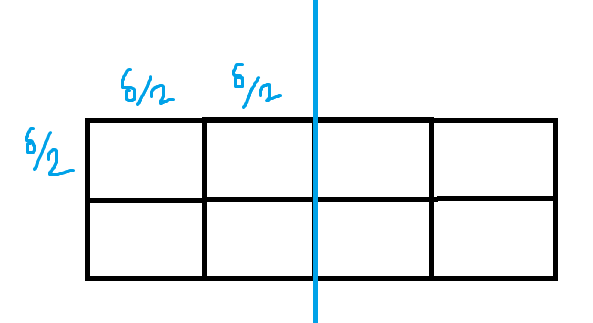
\includegraphics{D:/IIITD/Semester4/ADA/Pasted image 20220201144330.png}
  \item
    And also the box height is restricted by delta.
  \item
    bdmtish, drumroll, so, we only need to compare with points which may
    be in these boxes. Therefore a linear algo.
  \end{itemize}
\end{enumerate}

\hypertarget{lecture-5}{%
\section{Lecture\textrightarrow5}\label{lecture-5}}

\hypertarget{the-selection-problem}{%
\subsection{The selection problem}\label{the-selection-problem}}

Input: An array (arbitrary), an integer {\(i\)}\\
Goal: Get {\(i^{\text{th}}\)} smallest number or {\(i^{\text{th}}\)}
order statistic.

We'll see a linear time selection algo.

\begin{Shaded}
\begin{Highlighting}[]
\NormalTok{Select(A, length n, i)}
\NormalTok{    base: do something idk}
\NormalTok{    else:}
\NormalTok{        1. Choose any element as pivot = p}
\NormalTok{        2. Partition A around p (just like quicksort)}
\NormalTok{        3. Let j: position of p now}
\NormalTok{        4. if j==i then return P}
\NormalTok{        5. if j\textgreater{}i: recurse: return Select(A[1..j{-}1],j{-}1,i)}
\NormalTok{        6. if j\textless{}i: recurse: return Select(A[j+1..n], n{-}j, i{-}j)}
\NormalTok{Copy}
\end{Highlighting}
\end{Shaded}

Runtime:\\
We will analyze the worst case (i.e. we recurse on the larger subarray)

\begin{itemize}
\tightlist
\item
  {\(T(n) = c.n + T\lbrack\max(n - j,j - 1)\rbrack\)}
\item
  Worst case:
  {\(c \cdot n + c \cdot (n - 1) + c \cdot (n - 2)\cdots \in \mathcal{O}(cn^{2})\)}
\end{itemize}

So... \texttt{epic\ algorithm\ fail}.

\hypertarget{how-to-choose-a-good-pivot-fast}{%
\subsubsection{How to choose a good pivot
fast?}\label{how-to-choose-a-good-pivot-fast}}

Here are two choices

\begin{itemize}
\tightlist
\item
  Median (Best!) : But ...aren't you solving the median problem xD
\item
  {[}30\%-70\%{]} (Good enough)

  \begin{itemize}
  \tightlist
  \item
    Randomization: Choose pivot as any element \emph{uniformly at
    random}
  \item
    Theorem: RSelect works in \emph{expected} {\(\mathcal{O}(n)\)} time
  \item
    Deterministic pivot selection:

    \begin{itemize}
    \item
      Break array A into buckets of {\(5\)} elements (i.e. {\(K = n/5\)}
      groups)
    \item
      Find median of each group = {\(e\)} where {\(|e| = K\)}
    \item
      pivot {\(p = {Median}(e)\)}
    \item
      Let's re-write the algo:

\begin{Shaded}
\begin{Highlighting}[]
\NormalTok{DSelect(A,length n, i)}
\NormalTok{    base: idk}
\NormalTok{    else:}
\NormalTok{        1. Group A into chunks of 5}
\NormalTok{        2. e = set of medians from each}
\NormalTok{        3. p = DSelect( e, n/5 = K, K/2 )}
\NormalTok{        4. ...same as before}
\NormalTok{Copy}
\end{Highlighting}
\end{Shaded}
    \item
      Runtime analysis: We have {\(T(n) = c \cdot n + T(n/5) + T(?)\)}

      \begin{itemize}
      \tightlist
      \item
        Key lemma: Median of {\(e\)} is bigger than (and also smaller
        than) atleast 30\% of the set
      \item
        Proof:\\
        Visualize the array as a 2D grid.\\
        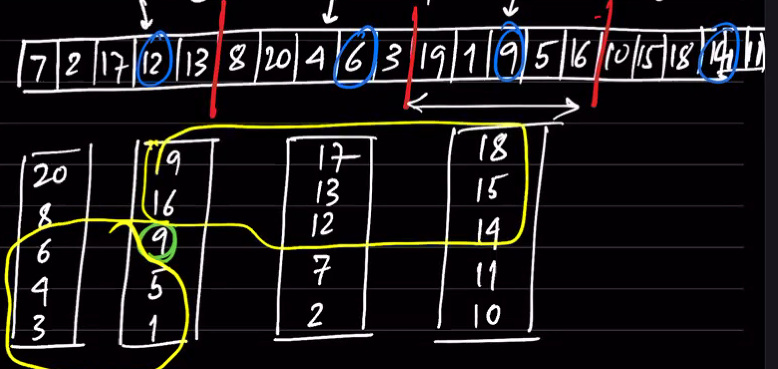
\includegraphics{D:/IIITD/Semester4/ADA/Pasted image 20220204144057.png}\\
        Here, pivot is {\(9\)}. now, let's generalize.
      \end{itemize}

      We have the recurrence
      {\(T(n) \leq c \cdot n + T(n/5) + T(0.7 \cdot n)\)}
    \end{itemize}
  \end{itemize}
\end{itemize}

\end{document}
